\documentclass[11pt,a4paper]{article}

\usepackage[utf8]{inputenc}
\usepackage[T1]{fontenc}
\usepackage{lmodern}
\usepackage[french]{babel}
\usepackage[margin=2.2cm]{geometry}
\usepackage{amsmath,amssymb}
\usepackage{booktabs,tabularx,array,multirow}
\usepackage{graphicx}
\usepackage[table]{xcolor}
\usepackage{tikz}
\usetikzlibrary{arrows.meta,positioning,shapes.geometric}
\usepackage{tcolorbox}
\tcbuselibrary{skins,breakable}
\usepackage{enumitem}
\usepackage{caption}
\usepackage{float}
\usepackage{fancyhdr}
\usepackage[hidelinks]{hyperref}

\graphicspath{{../reports/figures/}}

\definecolor{bleu}{HTML}{1F4E79}
\definecolor{bleuclair}{HTML}{E8F0F8}
\definecolor{vert}{HTML}{2E7D32}
\definecolor{vertclair}{HTML}{E8F5E9}
\definecolor{orange}{HTML}{E65100}
\definecolor{orangeclair}{HTML}{FFF3E0}
\definecolor{gris}{HTML}{F5F5F5}

\newtcolorbox{resume}[1][]{colback=bleuclair,colframe=bleu,fonttitle=\bfseries,title=#1,breakable}
\newtcolorbox{constat}[1][]{colback=vertclair,colframe=vert,fonttitle=\bfseries,title=#1,breakable}
\newtcolorbox{attention}[1][]{colback=orangeclair,colframe=orange,fonttitle=\bfseries,title=#1,breakable}

\newcommand{\best}[1]{\textbf{#1}}
\setlist{itemsep=2pt,topsep=4pt}
\renewcommand{\arraystretch}{1.18}

\pagestyle{fancy}
\fancyhf{}
\lhead{\small Projet CAMELYON17 — point d'avancement}
\rhead{\small \thepage}
\setlength{\headheight}{14pt}

\title{\vspace{-1.2cm}\textbf{\color{bleu}Projet CAMELYON17}\\[4pt]
\large Détection de métastases ganglionnaires et stade pN du cancer du sein\\[2pt]
\normalsize Point d'avancement complet pour l'équipe}
\author{Ali Houaoui}
\date{5 novembre 2026 — rendu prévu le 27/11/2026}

\begin{document}
\maketitle
\thispagestyle{fancy}

\begin{resume}[En une page : où on en est]
\begin{itemize}
  \item \textbf{Objectif} : à partir des lames de ganglions (images de microscope), (1) dire si un morceau d'image
        contient du cancer, puis (2) donner le \emph{stade pN} de chaque patiente (pN0, pN0(i+), pN1mi, pN1, pN2).
  \item \textbf{Étape 1 faite} — détection sur patchs : le meilleur choix est un \emph{modèle de fondation} en
        pathologie (Phikon) figé + régression logistique. Sur un hôpital jamais vu (centre 2) : AUC 0,990,
        sensibilité 0,98. Le ResNet18 classique ne rattrape que 69\,\% des tumeurs de cet hôpital.
  \item \textbf{Étape 2 faite} — stade pN sur 57 patientes jamais vues : kappa (métrique officielle)
        \begin{itemize}
          \item règle de taille 0,80 ; forêt aléatoire 0,80 (méthodes « type challenge ») ;
          \item \textbf{ABMIL hybride 0,887} (meilleur dans 10 répétitions sur 10, gain +0,08 [0,01 ; 0,18]) ;
          \item combinaison exploratoire « ET forêt » 0,892, macro-métastases ratées 2,1 $\to$ 0,3 (à confirmer).
        \end{itemize}
  \item \textbf{Point faible} : les petites métastases (micro, ITC). Hypothèse principale : notre résolution
        (1 µm/pixel) est 4 fois plus grossière que celle des gagnants du challenge.
  \item \textbf{Reste à faire} : interprétabilité, changement de domaine (partie notée), éthique, éventuellement une
        relecture à plus haute résolution des zones suspectes, puis rapport (15 p.) et oral (10 min).
\end{itemize}
\end{resume}

\tableofcontents
\newpage

%=====================================================================
\section{Le projet en bref}
%=====================================================================

\subsection{Le problème médical}
Dans le cancer du sein, on retire les ganglions lymphatiques de l'aisselle pour savoir si le cancer s'y est propagé.
Chaque ganglion est coupé, coloré (coloration \textbf{H\&E} : noyaux violets, cytoplasme rose) et numérisé en une
\emph{lame entière} (\emph{whole slide image}, WSI) : une image d'environ $100\,000 \times 200\,000$ pixels, 1 à 3\,Go.
Un pathologiste cherche des cellules tumorales et \textbf{mesure la taille de la plus grande métastase} :

\begin{table}[H]
\centering
\begin{tabular}{lll}
\toprule
\textbf{Classe d'un ganglion} & \textbf{Taille de la plus grande lésion} & \textbf{Sens} \\
\midrule
négatif & aucune cellule tumorale & sain \\
ITC (cellules tumorales isolées) & $< 0{,}2$ mm & quelques cellules \\
micro-métastase & $0{,}2$ à $2$ mm & petite métastase \\
macro-métastase & $> 2$ mm & métastase installée \\
\bottomrule
\end{tabular}
\caption{Classes d'un ganglion (règles TNM).}
\end{table}

Puis, à partir des 5 ganglions d'une patiente, il donne le \textbf{stade pN} :

\begin{table}[H]
\centering
\begin{tabular}{ll}
\toprule
\textbf{Stade pN} & \textbf{Règle (challenge CAMELYON17)} \\
\midrule
pN0 & aucun ganglion atteint \\
pN0(i+) & seulement des ITC \\
pN1mi & au moins une micro-métastase, aucune macro \\
pN1 & 1 à 3 ganglions atteints dont au moins une macro \\
pN2 & 4 à 9 ganglions atteints dont au moins une macro \\
\bottomrule
\end{tabular}
\caption{Du ganglion au stade de la patiente.}
\end{table}

Ce stade décide du traitement (chimiothérapie, radiothérapie, curage). Une erreur \emph{vers le bas} (métastase ratée)
est plus grave qu'une erreur \emph{vers le haut} (fausse alerte) : ce coût asymétrique guide tous nos choix de métriques.

\subsection{Objectif du travail}
\begin{enumerate}
  \item \textbf{Étape 1 — détection} : un modèle qui dit, pour chaque petit carré d'image (\emph{patch}, $96\times96$ pixels),
        s'il contient du tissu tumoral. Il doit marcher sur un \textbf{hôpital qu'il n'a jamais vu} (changement de domaine).
  \item \textbf{Étape 2 — stade} : appliquer ce détecteur à toute la lame pour obtenir une \emph{carte de chaleur},
        en déduire la classe de chaque ganglion, puis le stade pN de la patiente.
  \item \textbf{Étape 3 — recul critique} : interprétabilité, changement de domaine, éthique.
\end{enumerate}

\subsection{Livrables et notation}
Code sur GitHub (dépôt privé \texttt{alihouaoui/Projet\_Camelyon17}), rapport de 15 pages, oral de 10 minutes,
rendu vers le 27/11/2026.

\begin{table}[H]
\centering
\begin{tabular}{lr}
\toprule
\textbf{Critère} & \textbf{Poids} \\
\midrule
Suivi (journal, régularité) & 20\,\% \\
Données (exploration, découpage, qualité) & 25\,\% \\
Modèles & 25\,\% \\
Interprétabilité / changement de domaine / éthique & 10\,\% \\
Oral & 20\,\% \\
\bottomrule
\end{tabular}
\end{table}

%=====================================================================
\section{Pourquoi CAMELYON17 ?}
%=====================================================================
\begin{itemize}
  \item \textbf{Problème clinique réel et bien défini} : la tâche du challenge (stade pN) est exactement celle du pathologiste,
        avec des règles médicales officielles. On peut donc construire le stade comme lui, et non le « deviner ».
  \item \textbf{5 hôpitaux néerlandais} (centres 0 à 4), avec scanners et colorations différents : c'est le cas d'école du
        \textbf{changement de domaine}, un critère noté du projet. Un modèle peut avoir l'air excellent dans son hôpital et
        s'effondrer ailleurs (on l'a observé, section~\ref{sec:etape1}).
  \item \textbf{Deux niveaux de données} : des patchs prêts à l'emploi (Camelyon17-WILDS) pour l'étape 1, et les lames
        entières avec les stades officiels pour l'étape 2.
  \item \textbf{Données publiques et références} : lames en accès libre sur AWS, résultats du challenge publiés
        (Bándi et al., 2019), benchmark WILDS (Koh et al., 2021) : on peut se situer.
  \item \textbf{Métrique officielle} (kappa quadratique) qui tient compte de la gravité des erreurs.
\end{itemize}

%=====================================================================
\section{Les données}
%=====================================================================

\subsection{Patchs Camelyon17-WILDS (étape 1)}
\begin{itemize}
  \item \textbf{455\,954 patchs} RGB de $96\times96$ pixels, au niveau 2 de la pyramide (environ 0,97\,µm par pixel,
        un patch couvre environ 93\,µm), étiquetés tumeur / non-tumeur à partir des contours dessinés par des pathologistes.
  \item Issus de \textbf{50 lames, 43 patientes, 5 hôpitaux} (10 lames par hôpital). Classes équilibrées par construction.
  \item Récupération : le serveur officiel (CodaLab) avait un certificat HTTPS expiré ; on a utilisé le miroir Hugging Face
        \texttt{wltjr1007/Camelyon17-WILDS} (21 fichiers parquet, 10,7\,Go), effectifs vérifiés identiques.
\end{itemize}

\paragraph{Exploration (notebook \texttt{01\_exploration.ipynb}).}
Aucune valeur manquante. \textbf{La couleur seule (6 statistiques) reconnaît l'hôpital dans 80\,\% des cas} (hasard : 20\,\%) :
le centre 2 est nettement plus violet et saturé. Les patchs tumoraux sont regroupés dans l'espace : deux patchs voisins sont
presque identiques, d'où l'obligation de découper \emph{par patiente}.

\begin{figure}[H]
\centering
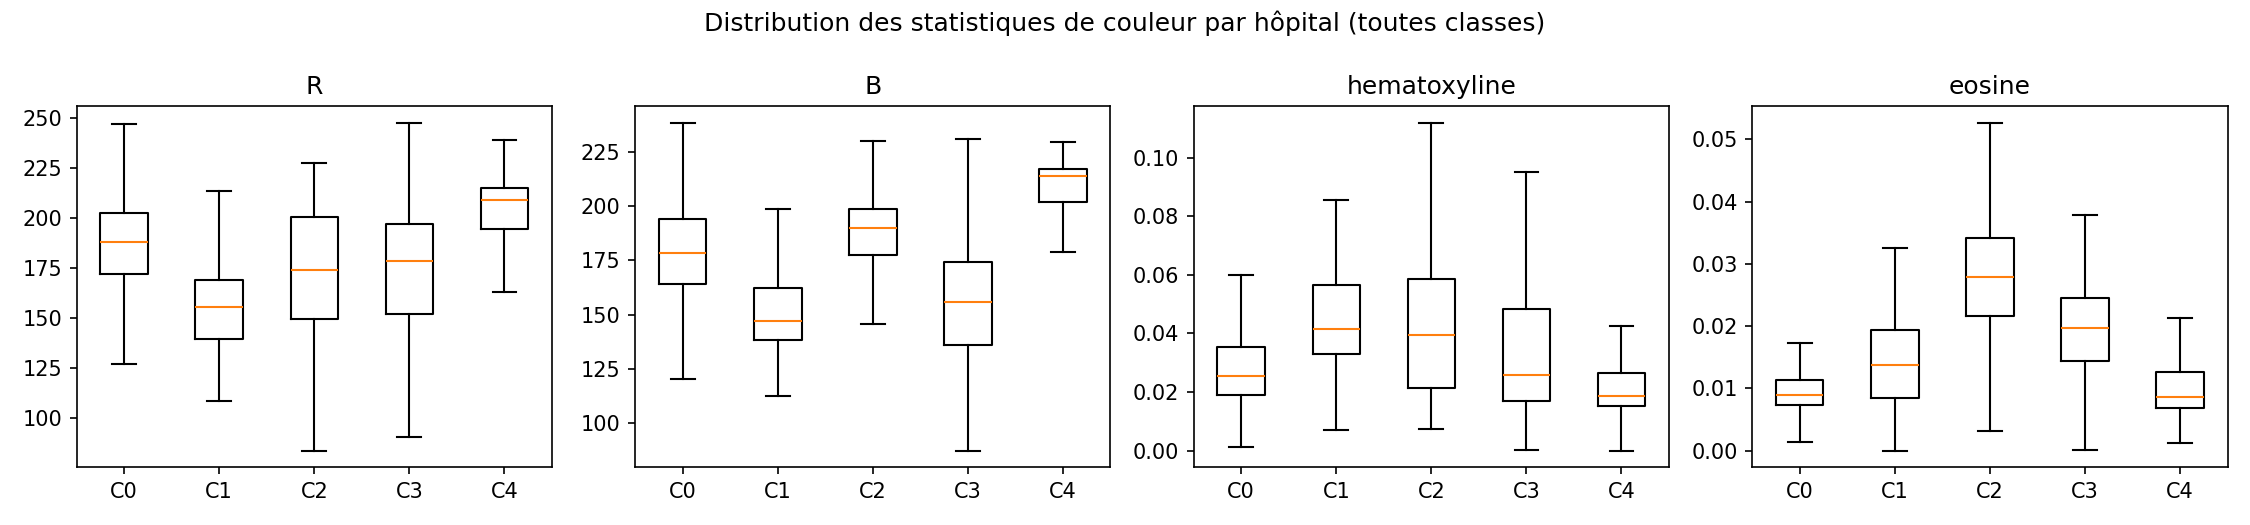
\includegraphics[width=0.48\textwidth]{couleur_par_centre.png}\hfill
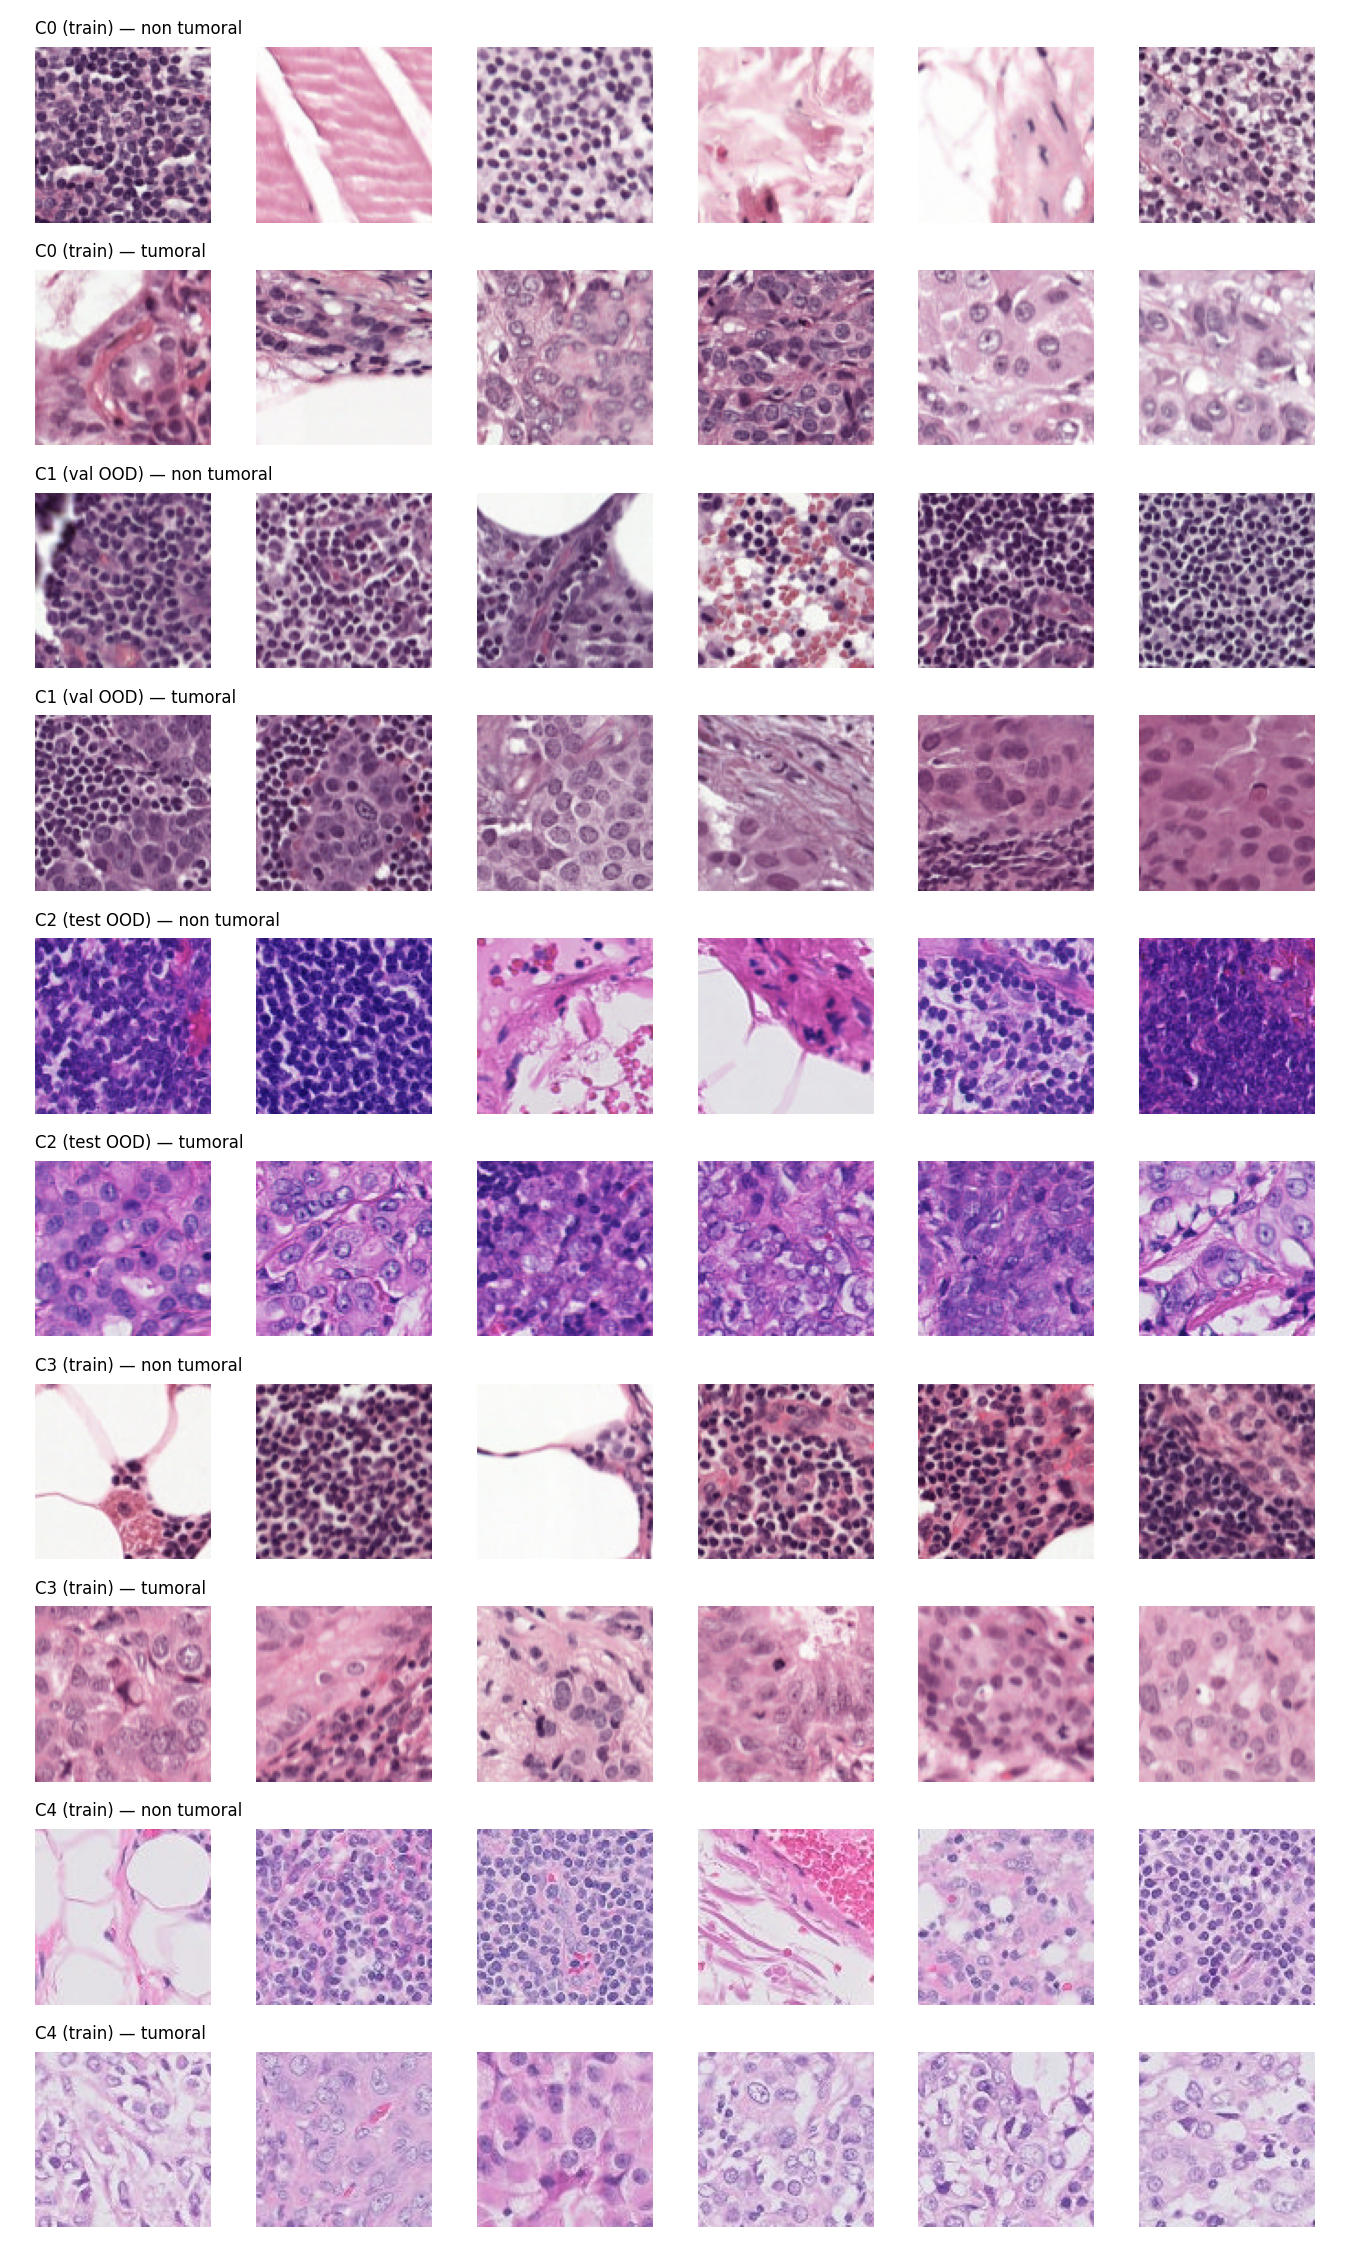
\includegraphics[width=0.48\textwidth]{galerie.png}
\caption{À gauche : la couleur diffère selon l'hôpital. À droite : exemples de patchs.}
\end{figure}

\subsection{Découpage sans fuite}
\begin{table}[H]
\centering
\begin{tabularx}{\textwidth}{llX}
\toprule
\textbf{Ensemble} & \textbf{Contenu} & \textbf{Usage} \\
\midrule
\texttt{train} & centres 0, 3, 4 — 80\,\% des patientes & apprentissage \\
\texttt{val\_id} & centres 0, 3, 4 — 20\,\% des patientes (autres) & choix du modèle et du seuil \\
\texttt{val\_ood} & centre 1 & généralisation à un hôpital inconnu \\
\texttt{test\_ood} & centre 2 & \textbf{test final, regardé une seule fois} \\
\bottomrule
\end{tabularx}
\caption{Découpage par patiente. Le split \texttt{id\_val} officiel de WILDS mélange des patchs des mêmes lames : écarté.
Une fonction (\texttt{check\_no\_leakage}) refuse tout découpage où une patiente apparaît deux fois.}
\end{table}

\subsection{Lames entières CAMELYON17 (étape 2)}
\begin{itemize}
  \item Source : bucket public AWS \texttt{s3://camelyon-dataset/CAMELYON17/}, avec le fichier officiel \texttt{stages.csv}
        (stade pN par patiente, classe par ganglion).
  \item \textbf{Cohorte : les 57 patientes dont le détecteur n'a jamais vu aucune image} (les 43 patientes WILDS sont exclues
        pour éviter toute fuite), 5 ganglions chacune, soit \textbf{285 lames} et environ \textbf{3 millions de tuiles}.
\end{itemize}

\begin{table}[H]
\centering
\begin{tabular}{lrrrrr|r}
\toprule
& pN0 & pN0(i+) & pN1mi & pN1 & pN2 & Total \\
\midrule
Patientes & 24 & 3 & 9 & 14 & 7 & 57 \\
\bottomrule
\end{tabular}
\quad
\begin{tabular}{lrrrr}
\toprule
Lames & négatives & ITC & micro & macro \\
\midrule
285 & 205 & 10 & 27 & 43 \\
\bottomrule
\end{tabular}
\caption{Cohorte de l'étape 2. Les petites classes (3 pN0(i+), 10 ITC) limitent la précision des conclusions.}
\end{table}

%=====================================================================
\section{Comment on fait tourner les calculs}
%=====================================================================

\begin{table}[H]
\centering
\begin{tabularx}{\textwidth}{lX}
\toprule
\textbf{Machine} & \textbf{Usage et astuces} \\
\midrule
Mac (CPU Intel/MPS, 12\,Go libres) & mise au point sur un échantillon de 40\,254 patchs ; ABMIL et stade pN (CPU) \\
Google Colab gratuit (GPU T4, 12,7\,Go RAM) & jeu complet, CNN, modèles de fondation, cartes de chaleur \\
\bottomrule
\end{tabularx}
\end{table}

\paragraph{Problèmes rencontrés et solutions.}
\begin{itemize}
  \item \textbf{Les 455\,954 images ne tiennent pas en RAM} : conversion unique en un fichier d'images décodées sur disque
        (\texttt{images.npy}, 12,6\,Go, lu à la demande par \emph{memmap}). Vérifié : pixels identiques.
  \item \textbf{Coupures de session Colab} (environ 1\,h de GPU) : points de sauvegarde (\texttt{best.pt}, \texttt{last.pt})
        rapatriés sur le Mac toutes les 4 minutes et reprise automatique.
  \item \textbf{2 cœurs CPU seulement} : les augmentations (symétries, rotations) faites par lot sur le GPU : 395 s $\to$ 250 s par époque.
  \item \textbf{Lames de 2\,Go} : on ne les télécharge pas. On lit l'en-tête TIFF puis \emph{seulement} les tuiles JPEG qui
        recouvrent du tissu, par requêtes HTTP « Range » parallèles (quelques \% du fichier).
  \item \textbf{Mémoire GPU saturée} sur les très grosses lames (34\,000 tuiles) : lot divisé par 2 automatiquement.
  \item \textbf{Lames Philips sans résolution dans l'en-tête} : lue dans la description XML ; une lame n'a que 7 niveaux.
  \item \textbf{Entraînements parallèles sur Mac} : 6 processus (\emph{spawn}, données partagées en memmap) car
        \emph{fork} se bloque avec PyTorch sur macOS.
\end{itemize}

\paragraph{Tailles de lot (batch) et réglages.}
\begin{table}[H]
\centering
\small
\begin{tabularx}{\textwidth}{lXXX}
\toprule
\textbf{Modèle} & \textbf{Batch} & \textbf{Optimiseur / pas} & \textbf{Durée} \\
\midrule
Petit CNN & 256 patchs & AdamW, OneCycle, lr $10^{-3}$, 5 époques & $\approx$ 250 s / époque (T4) \\
ResNet18 & 256 patchs & AdamW, OneCycle, lr $3\cdot10^{-4}$, 3 époques & $\approx$ 250 s / époque (T4) \\
Phikon (extraction) & 256 tuiles (réduit si saturé) & aucun (figé) & 20 min (WILDS) ; 1 lame/min (T4) \\
Sonde logistique & tout le jeu & régularisation par CV groupée & quelques minutes \\
ABMIL & 1 lame (« sac ») par pas & AdamW, lr $2\cdot10^{-4}$, 20 époques & $\approx$ 20 min / répétition \\
\bottomrule
\end{tabularx}
\end{table}

%=====================================================================
\section{Les métriques et à quoi elles servent}
%=====================================================================

\subsection{Étape 1 (patchs)}
\begin{itemize}
  \item \textbf{AUC} (aire sous la courbe ROC) : probabilité qu'un patch tumoral reçoive un score plus élevé qu'un patch sain.
        Mesure la capacité à \emph{classer}, indépendamment du seuil. 0,5 = hasard, 1 = parfait.
  \item \textbf{Sensibilité} $= \frac{VP}{VP+FN}$ : part des tumeurs détectées. \textbf{C'est la métrique prioritaire}
        (une tumeur ratée = une patiente sous-traitée).
  \item \textbf{Spécificité} $= \frac{VN}{VN+FP}$ : part des tissus sains correctement écartés (évite les fausses alertes,
        donc la charge de relecture).
  \item \textbf{Seuil à sensibilité 95\,\%} : on fixe le seuil sur les hôpitaux d'entraînement pour détecter 95\,\% des tumeurs,
        puis on l'applique \emph{tel quel} au nouvel hôpital. Cela teste si le modèle est \emph{utilisable} ailleurs, pas seulement
        s'il classe bien. Le seuil 0,5 est rapporté à côté.
  \item \textbf{Intervalle de confiance à 95\,\% par bootstrap des patientes} : on retire au hasard des patientes (et non des patchs,
        trop corrélés) 1\,000 fois ; cela montre si une différence entre modèles est solide ou due au hasard.
\end{itemize}

\subsection{Étape 2 (stade pN)}
\begin{itemize}
  \item \textbf{Kappa de Cohen pondéré quadratique} (métrique officielle du challenge) :
  \[
     \kappa = 1 - \frac{\sum_{i,j} w_{ij}\, O_{ij}}{\sum_{i,j} w_{ij}\, E_{ij}}, \qquad w_{ij} = \frac{(i-j)^2}{(K-1)^2}
  \]
  où $O$ est la matrice de confusion observée, $E$ celle attendue par hasard et $K=5$ stades. Une erreur de deux crans
  coûte 4 fois plus qu'une erreur d'un cran. 0 = hasard, 1 = accord parfait ; au-delà de 0,8 on parle d'accord « presque parfait ».
  \item \textbf{Stade exact} : pourcentage de patientes au bon stade (plus lisible, mais ignore la gravité).
  \item \textbf{Métriques cliniques} (en nombre de patientes sur 57) :
    \begin{itemize}
      \item \emph{métastatiques ratées} : patientes pN1mi/pN1/pN2 classées pN0 ou pN0(i+) ;
      \item \emph{macro ratées} : patientes pN1/pN2 classées en dessous de pN1 (\textbf{l'erreur la plus grave}) ;
      \item \emph{sur-stadification} : patientes pN0/pN0(i+) classées métastatiques (traitement inutile).
    \end{itemize}
  \item \textbf{Validation croisée répétée par patiente} : 3 plis (car seulement 3 patientes pN0(i+)), stratifiés sur le stade,
        répétés 10 à 20 fois avec des découpages différents. On donne la moyenne et le min–max : avec 57 patientes,
        un seul découpage peut faire varier le kappa de 0,69 à 0,87.
  \item \textbf{Écart de kappa apparié} : deux méthodes comparées sur exactement les mêmes plis, avec IC par bootstrap des patientes.
\end{itemize}

%=====================================================================
\section{Les architectures des modèles}
%=====================================================================

\subsection{Étape 1 : classifieurs de patchs}
\begin{description}[style=nextline]
  \item[Référence classique] statistiques de couleur et de texture (moyennes, écarts-types, histogrammes, textures LBP et matrices de co-occurrence)
        $\to$ régression logistique ou forêt aléatoire. Sert de point de comparaison « sans apprentissage profond ».
  \item[Petit CNN (appris de zéro)] 4 blocs \{convolution $3\times3$ $\to$ normalisation de lot $\to$ ReLU $\to$ max-pooling\},
        largeurs 32, 64, 128, 256, puis pooling global, dropout 0,3 et couche linéaire (2 classes).
  \item[ResNet18 pré-entraîné] réseau résiduel à 18 couches (11\,M paramètres) pré-entraîné sur ImageNet (photos), dernière couche
        remplacée et réseau entièrement ré-entraîné (\emph{fine-tuning}).
  \item[Modèles de fondation + sonde linéaire] un \emph{Vision Transformer} (ViT) pré-entraîné par auto-supervision sur des millions
        de patchs de pathologie, \textbf{figé} (on ne le ré-entraîne pas) : il transforme chaque patch (agrandi en $224\times224$)
        en un vecteur de caractéristiques. Puis une régression logistique (la « sonde ») décide tumeur / non-tumeur.
        \begin{itemize}
          \item \textbf{Phikon} (Owkin) : ViT-B/16, 86\,M paramètres, vecteur de 768, appris sur TCGA ;
          \item \textbf{Phikon-v2} : ViT-L, appris sur TCGA + CPTAC + GTEx ;
          \item \textbf{Midnight-12k} : ViT-g (plus d'un milliard de paramètres), appris sur TCGA ;
          \item \textbf{DINOv2-base} : même principe mais appris sur des photos ordinaires (contrôle).
        \end{itemize}
        Aucun n'a vu CAMELYON pendant son pré-entraînement (d'après leurs fiches).
\end{description}

\subsection{Étape 2 : du patch au stade}

\begin{figure}[H]
\centering
\begin{tikzpicture}[node distance=0.55cm and 0.5cm, every node/.style={font=\small},
  box/.style={draw=bleu, fill=bleuclair, rounded corners, align=center, minimum height=1.1cm, text width=2.3cm},
  arr/.style={-{Stealth[length=2.5mm]}, thick, bleu}]
\node[box] (wsi) {Lame entière\\(1 ganglion)};
\node[box, right=of wsi] (tiles) {Tuiles $96{\times}96$\\sur le tissu};
\node[box, right=of tiles] (phikon) {Phikon figé\\+ sonde};
\node[box, right=of phikon] (map) {Carte de chaleur\\$p(\text{tumeur})$};
\node[box, below=1.1cm of map, fill=vertclair, draw=vert] (cls) {Classe du ganglion\\(nég., ITC,\\micro, macro)};
\node[box, left=of cls, fill=vertclair, draw=vert] (pn) {Règles pN\\(5 ganglions)};
\node[box, left=of pn, fill=orangeclair, draw=orange] (stage) {Stade pN\\de la patiente};
\draw[arr] (wsi) -- (tiles); \draw[arr] (tiles) -- (phikon); \draw[arr] (phikon) -- (map);
\draw[arr] (map) -- node[right, align=left, font=\scriptsize]{règle de taille,\\forêt, ou ABMIL} (cls);
\draw[arr] (cls) -- (pn); \draw[arr] (pn) -- (stage);
\end{tikzpicture}
\caption{Chaîne de décision : le stade n'est pas « deviné » par un modèle, il est construit comme le fait le pathologiste.}
\end{figure}

\begin{description}[style=nextline]
  \item[1. Carte de chaleur] masque du tissu (seuil d'Otsu sur la saturation, sur une miniature), toutes les tuiles de $96\times96$
        du niveau 2 contenant au moins 25\,\% de tissu, encodées par Phikon puis notées par la sonde de l'étape 1.
  \item[2a. Règle de taille] on garde les tuiles au-dessus d'un seuil $t$, on regroupe les taches d'au moins $m$ tuiles et on mesure
        le plus grand diamètre (diamètre de Feret) en mm ; puis les seuils médicaux 0,2 et 2\,mm (non réglés). Seuls $t$ et $m$ sont appris.
        \emph{Avantage : entièrement explicable.}
  \item[2b. Forêt aléatoire] 300 arbres sur des résumés de la carte (probabilité max, moyenne des 10 meilleures tuiles, nombre de
        tuiles et plus grand diamètre aux seuils 0,5 / 0,9 / 0,99, quantité de tissu). C'est l'approche des gagnants du challenge.
  \item[2c. ABMIL (apprentissage multi-instances par attention)] une lame est un « sac » de milliers de vecteurs Phikon. Le modèle
        apprend lui-même quelles tuiles regarder (Ilse et al., 2018, attention à porte, environ 110\,k paramètres) :
        \[
          h_k = \mathrm{ReLU}(W x_k), \qquad z = \sum_k a_k h_k, \qquad \hat y = \mathrm{softmax}(C z),
        \]
        \[
          a_k = \frac{\exp\{w^\top(\tanh(V h_k) \odot \sigma(U h_k))\}}{\sum_j \exp\{w^\top(\tanh(V h_j) \odot \sigma(U h_j))\}}
        \]
        ($768 \to 128$, attention de dimension 64, dropout 0,25). Les poids $a_k$ donnent une carte d'attention.
        \begin{itemize}
          \item \textbf{ABMIL hybride (modèle principal)} : l'ABMIL décide seulement « ganglion atteint (micro/macro) ou non » ;
                la \emph{taille} vient de la règle. Raison : l'attention fait une moyenne pondérée, elle ne mesure pas une taille.
          \item \textbf{ABMIL 3 classes} (secondaire) : prédit directement négatif / micro / macro.
        \end{itemize}
        Entraînement : toutes les tuiles suspectes (sonde $\geq 0{,}3$) complétées au hasard jusqu'à 8\,000 tuiles par lame ;
        perte d'entropie croisée pondérée par classe ; prédiction sur toutes les tuiles.
  \item[3. Stade pN] application des règles officielles aux 5 ganglions (aucun modèle).
\end{description}

%=====================================================================
\section{Les résultats}
%=====================================================================

\subsection{Étape 1 : détection sur patchs, premiers modèles}\label{sec:etape1}
Seuil fixé sur \texttt{val\_id} pour 95\,\% de sensibilité, puis appliqué tel quel aux hôpitaux 1 et 2.

\begin{table}[H]
\centering
\footnotesize\setlength{\tabcolsep}{4pt}
\begin{tabular}{lcccccc}
\toprule
\textbf{Modèle} & \textbf{AUC val\_id} & \textbf{AUC C1} & \textbf{AUC C2} & \textbf{Sens. C2} & \textbf{Spéc. C2} & \textbf{Tumeurs C2 ratées} \\
\midrule
Couleur + texture, rég. log. & 0,973 & 0,838 & 0,660 & 0,63 & 0,62 & 37\,\% \\
Couleur + texture, forêt & 0,965 & 0,901 & 0,896 & 0,99 & 0,36 & 1\,\% \\
Petit CNN (5 époques) & 0,993 & 0,912 & 0,893 & 0,82 & 0,79 & 18\,\% \\
ResNet18 (3 époques) & \best{0,997} & \best{0,979} & \best{0,958} & 0,69 & \best{0,99} & 31\,\% \\
\bottomrule
\end{tabular}
\caption{Jeu complet (455\,954 patchs).}
\end{table}

\begin{constat}[Constat : un bon AUC ne suffit pas]
Le ResNet18 classe bien les patchs du centre 2 (AUC 0,958) mais \textbf{rate 31\,\% des tumeurs} (13\,183 sur 42\,527) au seuil appris
ailleurs : ses probabilités sont décalées par la couleur violette du centre 2. Il faudrait un seuil de 0,023 au lieu de 0,843.
Plus on l'entraîne, plus il se spécialise sur ses hôpitaux (AUC C1 : 0,983 $\to$ 0,958 entre les époques 1 et 3).
\end{constat}

\subsection{Étape 1 : modèles de fondation (figés + sonde)}
Régularisation et seuil choisis par validation croisée groupée par patiente sur les centres 0, 3, 4 (corrige la faiblesse
de \texttt{val\_id}, dominé par 2 patientes).

\begin{table}[H]
\centering
\footnotesize\setlength{\tabcolsep}{4pt}
\begin{tabular}{lcccr}
\toprule
\textbf{Modèle (centre 2, 9 patientes)} & \textbf{AUC [IC 95\,\%]} & \textbf{Sensibilité [IC 95\,\%]} & \textbf{Spécificité} & \textbf{Tumeurs ratées} \\
\midrule
Petit CNN & 0,893 [0,74–0,94] & 0,82 [0,48–0,92] & 0,79 & 7\,808 \\
ResNet18 fine-tuné & 0,958 [0,89–0,98] & 0,69 [0,28–0,80] & 0,99 & 13\,183 \\
DINOv2 générique, figé & 0,977 [0,95–0,98] & 0,96 [0,90–0,97] & 0,86 & 1\,792 \\
\rowcolor{bleuclair} \textbf{Phikon, figé} & 0,990 [0,97–0,99] & \best{0,98} [0,95–0,99] & 0,83 & 705 \\
Phikon-v2, figé & 0,989 [0,96–1,00] & 0,97 [0,90–0,99] & 0,95 & 1\,322 \\
Midnight-12k, figé (100\,k patchs) & \best{0,996} [0,99–1,00] & 0,96 [0,90–0,98] & \best{1,00} & 391 / 18\,655 \\
\bottomrule
\end{tabular}
\end{table}

\begin{figure}[H]
\centering
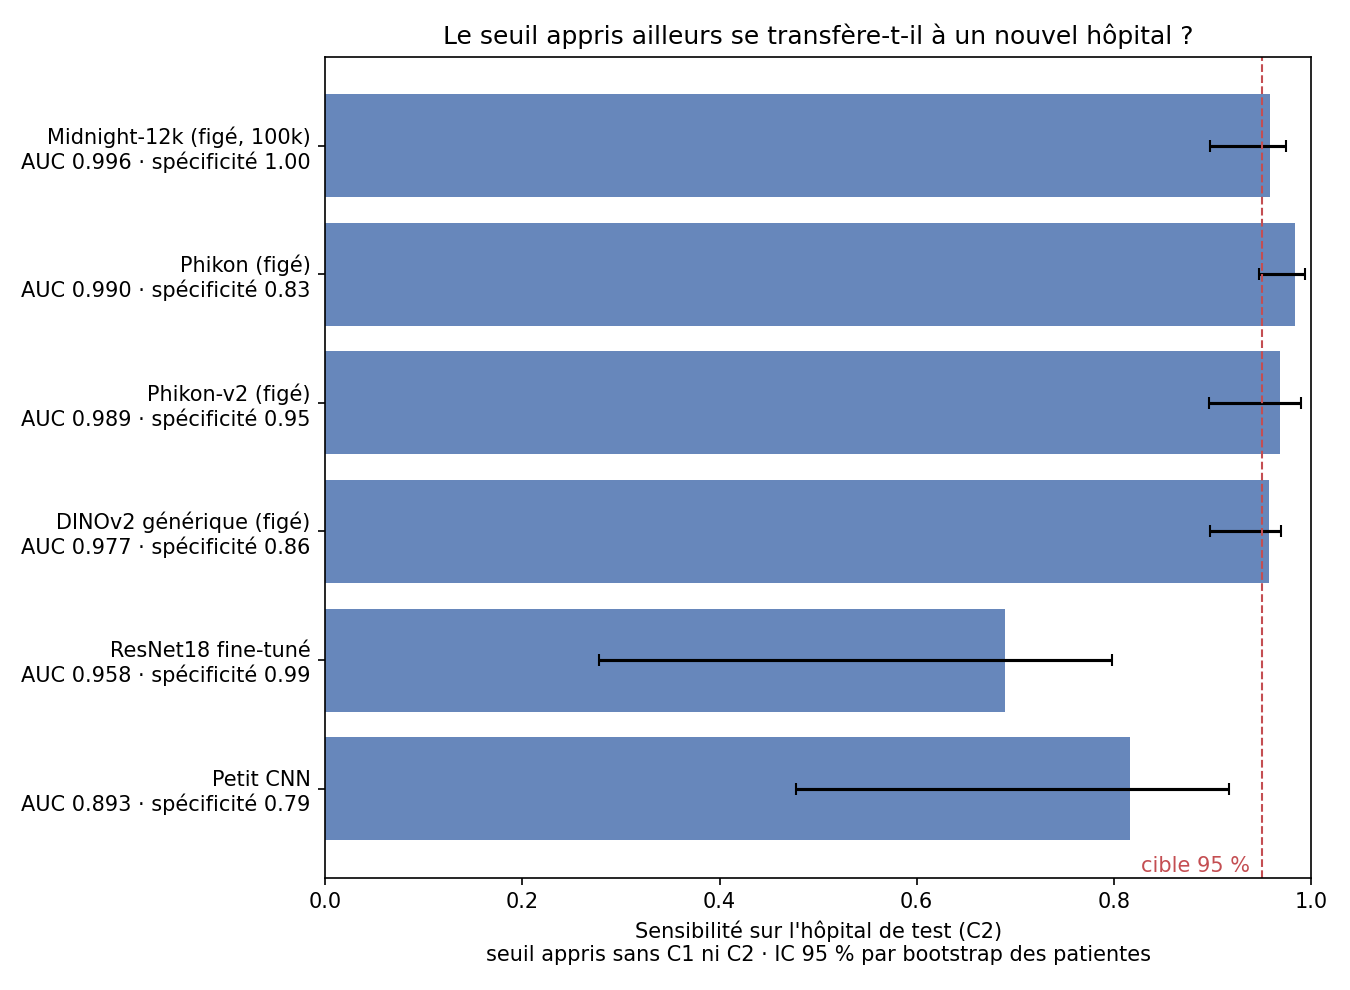
\includegraphics[width=0.75\textwidth]{sensibilite_c2.png}
\caption{Sensibilité sur le centre 2 au seuil appris ailleurs.}
\end{figure}

\begin{constat}[Constats]
\begin{enumerate}
  \item Avec les modèles de pathologie, \textbf{le seuil se transfère} : réglé à 95\,\% sur les hôpitaux d'entraînement, il donne
        95–98\,\% sur les hôpitaux 1 et 2. Le ResNet18 tombe à 69\,\% avec un IC très large (28–80\,\%).
  \item Une simple régression logistique sur des caractéristiques figées bat un ResNet18 entraîné de bout en bout.
  \item Le pré-entraînement \emph{en pathologie} compte : DINOv2 transfère aussi, mais avec plus de fausses alertes.
  \item Phikon, Phikon-v2 et Midnight ont des IC qui se chevauchent : pas de vainqueur net. \textbf{Phikon a été retenu pour
        l'étape 2} car il est rapide (20 min contre plusieurs heures pour Midnight sur 3 millions de tuiles).
\end{enumerate}
\end{constat}

\subsection{Étape 2 : stade pN (57 patientes jamais vues)}

\begin{figure}[H]
\centering
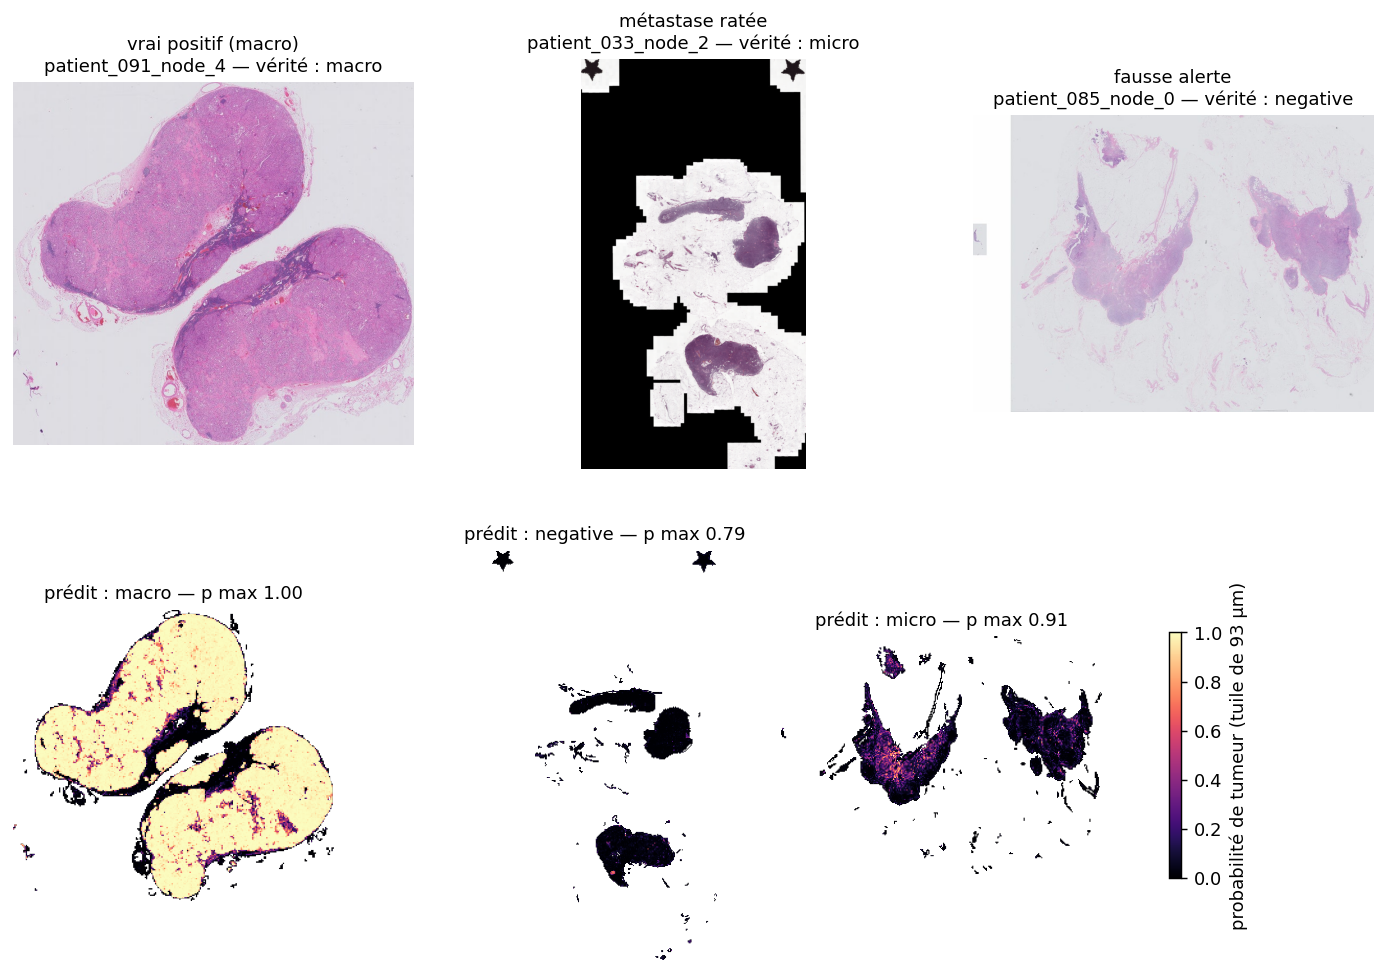
\includegraphics[width=0.95\textwidth]{pn_cartes_exemples.png}
\caption{Cartes de chaleur : vrai positif, métastase ratée, fausse alerte.}
\end{figure}

\begin{table}[H]
\centering
\footnotesize\setlength{\tabcolsep}{4pt}
\begin{tabular}{lccccc}
\toprule
\textbf{Méthode (étape 2)} & \textbf{Kappa (min–max)} & \textbf{pN exact} & \textbf{Métast. ratées} & \textbf{Macro ratées} & \textbf{Sur-stadif.} \\
\midrule
Règle de taille & 0,80 (0,77–0,83) & 69\,\% & 6,4 & 2,1 & 5,4 \\
Forêt aléatoire & 0,80 (0,76–0,87) & 69\,\% & 6,3 & 0,5 & 4,4 \\
ABMIL 3 classes & 0,87 (0,85–0,91) & 78\,\% & 5,1 & 1,3 & \best{1,2} \\
\rowcolor{bleuclair} \textbf{ABMIL hybride} & \best{0,887} (0,86–0,93) & 79\,\% & \best{4,4} & 2,1 & 1,5 \\
ABMIL hybride, 3 graines & 0,882 (0,86–0,90) & 78\,\% & 4,8 & 2,1 & 1,4 \\
\midrule
\textit{Explo. : OU forêt} & 0,866 (0,84–0,89) & 79\,\% & 4,1 & \best{0,3} & 2,4 \\
\textit{Explo. : ET forêt} & \best{0,892} (0,88–0,91) & \best{81\,\%} & 4,8 & \best{0,3} & 1,4 \\
\bottomrule
\end{tabular}
\caption{3 plis $\times$ 10 répétitions, mêmes plis pour toutes les méthodes. Métriques cliniques en nombre moyen de patientes sur 57.
« OU » : macro si la forêt dit macro ; « ET » : macro si la forêt dit macro \emph{et} l'ABMIL dit atteint.}
\end{table}

\begin{table}[H]
\centering
\small
\begin{tabular}{llc}
\toprule
\textbf{Statut} & \textbf{Comparaison} & \textbf{Écart de kappa [IC 95\,\%]} \\
\midrule
confirmatoire & ABMIL hybride $-$ règle & $+0{,}086$ [$0{,}015$ ; $0{,}178$] \\
confirmatoire & ABMIL hybride $-$ forêt & $+0{,}083$ [$0{,}012$ ; $0{,}177$] \\
secondaire & ABMIL 3 classes $-$ règle & $+0{,}074$ [$-0{,}002$ ; $0{,}162$] \\
confirmatoire & 3 graines $-$ 1 graine & $-0{,}005$ [$-0{,}016$ ; $0{,}003$] \\
exploratoire & OU forêt $-$ hybride 3 graines & $-0{,}016$ [$-0{,}080$ ; $0{,}025$] \\
exploratoire & ET forêt $-$ hybride 3 graines & $+0{,}010$ [$0{,}002$ ; $0{,}020$] \\
\bottomrule
\end{tabular}
\caption{Écarts appariés. Un IC qui exclut 0 indique une différence solide.}
\end{table}

\begin{constat}[Constats de l'étape 2]
\begin{enumerate}
  \item \textbf{L'ABMIL hybride bat la règle et la forêt dans 10 répétitions sur 10} (+0,08 de kappa). Le gain vient de la
        détection des petites métastases et de 3 fois moins de fausses alertes.
  \item La forêt rate moins de macro-métastases (0,5 contre 2,1) : d'où l'idée de les combiner. La version « ET » garde le meilleur
        des deux (0,3 macro ratée, pas plus de fausses alertes) mais elle a été imaginée \emph{après} avoir vu les résultats :
        \textbf{exploratoire, à confirmer sur d'autres données}.
  \item Moyenner 3 graines n'apporte rien (résultat négatif) : on garde une seule graine.
  \item \textbf{Relecture humaine} des patientes où ABMIL et forêt ne sont pas d'accord : 12,7 patientes sur 57 (22\,\%) à relire ;
        parmi les autres, il reste 4,0 métastatiques ratées mais seulement 0,3 macro ratée.
  \item \textbf{Point faible commun : les micro-métastases et ITC.} Aucune ITC détectée (plus petite qu'une tuile de 93\,µm) ;
        4 à 5 pN1mi classées pN0. Les cancers avancés sont bien classés.
\end{enumerate}
\end{constat}

\paragraph{Repère.} Les meilleures équipes du challenge CAMELYON17 atteignaient un kappa de l'ordre de 0,9 ou plus sur le jeu de test officiel (100 patientes, 500 lames).
\textbf{Ce n'est pas directement comparable} : nous travaillons en validation croisée sur 57 patientes, à une résolution 4 fois plus faible.

%=====================================================================
\section{Ce que font les autres projets sur cette base}
%=====================================================================
\begin{itemize}
  \item \textbf{Gagnants du challenge} (Bándi et al., 2019) : même chaîne que nous (détecteur $\to$ carte de chaleur $\to$ résumés
        $\to$ forêt / boosting $\to$ règles pN), mais à \textbf{pleine résolution} (0,24\,µm/pixel), avec réentraînement sur les erreurs
        (\emph{hard negative mining}) et réseau ajusté. Eux aussi ratent presque toutes les ITC.
  \item \textbf{Apprentissage multi-instances} évalué sur CAMELYON16 : CLAM (Lu, 2021), TransMIL (Shao, 2021), DSMIL (Li, 2021),
        DTFD-MIL (Zhang, 2022). Avec un bon encodeur, ils font à peu près jeu égal avec l'ABMIL.
  \item \textbf{Modèles de fondation récents} : UNI/UNI2, CONCH, Virchow2, H-optimus, Prov-GigaPath, souvent meilleurs que Phikon
        (accès sous licence sur Hugging Face).
  \item \textbf{Camelyon17-WILDS} : augmentation de couleur, normalisation de coloration, généralisation entre hôpitaux.
\end{itemize}

%=====================================================================
\section{Ce qu'on va probablement choisir, et pourquoi}
%=====================================================================

\begin{table}[H]
\centering
\begin{tabularx}{\textwidth}{lX}
\toprule
\textbf{Choix} & \textbf{Pourquoi} \\
\midrule
Phikon figé + sonde logistique (étape 1) & seuil qui se transfère à un hôpital inconnu, meilleure sensibilité, rapide ;
  le ResNet18 montre bien le piège du changement de domaine \\
ABMIL hybride (étape 2, modèle principal) & choisi \emph{avant} les résultats, meilleur dans 10/10 répétitions, IC qui exclut 0,
  et reste explicable (la taille vient d'une règle médicale) \\
Règle de taille (référence) & entièrement explicable, sert de base honnête \\
« ET forêt » (en ouverture) & meilleur sur les macro, mais exploratoire : présenté comme piste à confirmer \\
\bottomrule
\end{tabularx}
\end{table}

\paragraph{Pistes pour aller plus loin (à discuter en équipe).}
\begin{enumerate}
  \item \textbf{Relire à plus haute résolution (niveau 1 ou 0) seulement les zones suspectes} — ce qui nous sépare le plus des gagnants,
        ciblé sur nos micro-métastases ratées. Coût moyen.
  \item Changer d'encodeur (UNI ou CONCH) — gain moyen, coût élevé (recalculer 3 millions de tuiles).
  \item CLAM ou TransMIL à la place de l'ABMIL — gain probablement faible.
\end{enumerate}

%=====================================================================
\section{Reste à faire et répartition proposée}
%=====================================================================
\begin{table}[H]
\centering
\begin{tabularx}{\textwidth}{lXl}
\toprule
\textbf{Tâche} & \textbf{Contenu} & \textbf{Pour} \\
\midrule
Interprétabilité & cartes d'attention de l'ABMIL contre cartes de la sonde sur les pN1mi ratées ; Grad-CAM sur les faux
  négatifs du ResNet18 & semaine 3 \\
Changement de domaine & résultats par hôpital, augmentation HED / normalisation de couleur, éventuellement t-SNE ou VAE & semaine 3 \\
Éthique & outil d'aide et non de remplacement, coût asymétrique des erreurs, relecture humaine des lames négatives,
  biais (5 hôpitaux néerlandais), confidentialité & semaine 3 \\
Résolution (option) & relecture à plus haute résolution des zones suspectes & selon le temps \\
Rapport (15 p.) & contexte, données, méthodes, résultats, discussion, perspectives & semaine 4 \\
Oral (10 min) & diapositives, répétition & semaine 4 \\
\bottomrule
\end{tabularx}
\end{table}

\begin{attention}[Limites à toujours rappeler]
\begin{itemize}
  \item 57 patientes seulement : chiffres instables (kappa de 0,69 à 0,87 selon le découpage), encore plus par hôpital.
  \item Les réglages sont choisis dans la validation croisée, pas sur un jeu de test séparé.
  \item La « vérité » de taille des pathologistes vient de l'immunohistochimie (IHC), que le modèle ne voit pas (H\&E seulement).
  \item Le centre 2 a été regardé pour 6 modèles à l'étape 1 : résultats descriptifs.
  \item L'attention de l'ABMIL n'est pas une explication causale.
\end{itemize}
\end{attention}

%=====================================================================
\section{Où trouver quoi dans le dépôt}
%=====================================================================
\begin{table}[H]
\centering
\small
\begin{tabularx}{\textwidth}{lX}
\toprule
\textbf{Fichier} & \textbf{Rôle} \\
\midrule
\texttt{JOURNAL.md} & décisions et résultats, séance par séance \\
\texttt{notebooks/01\_exploration.ipynb} & exploration des données \\
\texttt{notebooks/02\_colab.ipynb} & chaîne complète sur Colab \\
\texttt{src/data.py}, \texttt{src/metrics.py} & chargement, découpage sans fuite, métriques \\
\texttt{src/models.py}, \texttt{scripts/train\_cnn.py} & petit CNN et ResNet18 \\
\texttt{src/foundation.py}, \texttt{scripts/linear\_probe.py} & modèles de fondation et sonde \\
\texttt{src/wsi.py}, \texttt{scripts/wsi\_features.py} & lecture à distance des lames, cartes de chaleur \\
\texttt{scripts/pn\_stage.py} & règle de taille, forêt, stade pN \\
\texttt{scripts/pn\_abmil.py}, \texttt{scripts/pn\_ensemble.py} & ABMIL, graines, combinaisons \\
\texttt{reports/} & tableaux de résultats (CSV) et figures \\
\bottomrule
\end{tabularx}
\end{table}

\section*{Glossaire}
\begin{description}[leftmargin=3.2cm, style=sameline, font=\bfseries]
  \item[Patch / tuile] petit carré d'image ($96\times96$ pixels, environ 93\,µm).
  \item[WSI] lame entière numérisée, pyramide de résolutions (niveau 0 = pleine résolution).
  \item[Changement de domaine] baisse de performance quand on change d'hôpital (scanner, coloration).
  \item[Modèle de fondation] grand réseau pré-entraîné sans étiquettes sur des millions d'images, réutilisé tel quel.
  \item[Sonde linéaire] régression logistique posée sur les caractéristiques d'un modèle figé.
  \item[MIL / ABMIL] apprentissage où l'étiquette est donnée pour un sac (une lame) et non pour chaque tuile.
  \item[Kappa quadratique] accord entre deux classements ordonnés, pénalisant fortement les grosses erreurs.
  \item[Bootstrap] ré-échantillonnage répété pour estimer l'incertitude.
\end{description}

\section*{Références}
\small
Bándi P. et al. (2019). \emph{From detection of individual metastases to classification of lymph node status at the patient level:
the CAMELYON17 challenge}. IEEE TMI.\\
Koh P.W. et al. (2021). \emph{WILDS: a benchmark of in-the-wild distribution shifts}. ICML.\\
Ilse M., Tomczak J., Welling M. (2018). \emph{Attention-based deep multiple instance learning}. ICML.\\
Filiot A. et al. (2023). \emph{Scaling self-supervised learning for histopathology with masked image modeling} (Phikon).\\
Tellez D. et al. (2019). \emph{Quantifying the effects of data augmentation and stain color normalization}. Medical Image Analysis.\\
Lu M.Y. et al. (2021). \emph{Data-efficient and weakly supervised computational pathology on whole-slide images} (CLAM). Nature BME.

\end{document}
